\documentclass[12pt]{article}
\usepackage[english]{babel}
\usepackage{natbib}
\usepackage{url}
\usepackage[utf8x]{inputenc}
\usepackage{amsmath}
\usepackage{graphicx}
\graphicspath{{img/}}
\usepackage{listings}
\usepackage{parskip}
\usepackage{fancyhdr}
\usepackage{vmargin}
\setmarginsrb{3 cm}{2.5 cm}{3 cm}{2.5 cm}{1 cm}{1.5 cm}{1 cm}{1.5 cm}

\title{Lab Report on \\ Basic GUI Control Elements in Matlab.}								% Title
\author{Rabi Raj Khadka}								% Author
\date{\today}											% Date


\makeatletter
\let\thetitle\@title
\let\theauthor\@author
\let\thedate\@date
\makeatother

\pagestyle{fancy}
\fancyhf{}
\rhead{\theauthor}
\lhead{\thetitle}
\cfoot{\thepage}

\begin{document}

%%%%%%%%%%%%%%%%%%%%%%%%%%%%%%%%%%%%%%%%%%%%%%%%%%%%%%%%%%%%%%%%%%%%%%%%%%%%%%%%%%%%%%%%%

\begin{titlepage}
	\centering
   % \vspace*{0.5 cm}
    
\includegraphics[scale = 0.3]{kheclogo.jpg}\\[1.0 cm]	% University Logo
    \textsc{\LARGE Khwopa Engineering College}\\[1.5 cm]	% University Name
	\textsc{\Large Course Code :BEG 475 IP}\\[0.5 cm]				% Course Code
	\textsc{\large Image Processing and Pattern recogntiion}\\[0.5 cm]				% Course Name
	\rule{\linewidth}{0.2 mm} \\[0.4 cm]
	{ \huge \bfseries \thetitle}\\
	\rule{\linewidth}{0.2 mm} \\[1.0 cm]
	
	% \texttt{Lab Report \#1}
	
	\rule{\linewidth}{0 mm} \\[1.0 cm]

	\begin{minipage}{0.4\textwidth}
		\begin{flushleft} \large
			\emph{Author:}\\
			\theauthor
			\end{flushleft}
			\end{minipage}~
			\begin{minipage}{0.4\textwidth}
			\begin{flushright} \large
			\emph{Roll  Number:} \\
			700324									% Your Student Number
		\end{flushright}
	\end{minipage}\\[2cm]
	
	{\large \thedate}\\[2 cm]
 
	\vfill
	
\end{titlepage}

%%%%%%%%%%%%%%%%%%%%%%%%%%%%%%%%%%%%%%%%%%%%%%%%%%%%%%%%%%%%%%%%%%%%%%%%%%%%%%%%%%%%%%%%%

\tableofcontents
\pagebreak
\section{Theory}
Basic GUI controls are as follows:\\\\
1.CheckBox:\\
A checkbox  is a GUI widget that permits the user to make a binary choice, i.e. a choice between one of two possible mutually exclusive options. For example, the user may have to answer 'yes' (checked) or 'no' (not checked) on a simple yes/no question.
Checkboxes are often shown on the screen as a square box that can contain white space in which the tick mark appears after selecting the checkbox.
 
2.Radio Button:\\
A radio button or option button is a graphical control element that allows the user to choose only one of a predefined set of mutually exclusive options. The singular property of a radio button makes it distinct from a checkbox, which allows more than one (or no) item to be selected and for the unselected state to be restored.
Radio buttons are arranged in groups of two or more and displayed on screen as, for example, a list of circular holes that can contain white space (for unselected) or a dot (for selected). The choices are mutually exclusive; when the user selects a radio button, any previously selected radio button in the same group becomes deselected (making it so only one can be selected).\\\\

Basic functions used for implementation of GUI in matlab are as follows:\\\\
1.$function btngroup_Callback(hObject, eventdata, handles)$\\
In this function the control of the button added on the GUI is done i.e we can easily modify and add the working of the button i.e what action to be done when the button is pressed, etc.\\
For eg:IPPR=get(handles.chkip,'Value')\\
If we write this code, the value of the checkbox chkip is copied to the variable IPPR. In this way we can implement this function.\\\\

2.$function pnlselect_SelectionChangedFcn(hObject, eventdata, handles)$\\
This function is the function for the panel that is added on the GUI. We can perform various functions from this function according to the requirement.\\
For eg: test=get(handles.pnlselect,'SelectedObject');\\
This code simply gets the selected object from the panel that is added in the GUI. In this way we can add codes for the selected panel also.

\pagebreak
\section{Code Description}
\lstinputlisting[language=Matlab]{labfour_Edited.m}
\pagebreak
\section{Result and Discussion}
We got to learn about various functions of GUI used in matlab and we were able to make a GUI that worked effectively. We also used various GUI widget like CheckBox, Radio Button, Panel, Push Button Etc.\\\\
The outputs of our GUI are as shown in figure below:\\\\
\emph{Output}

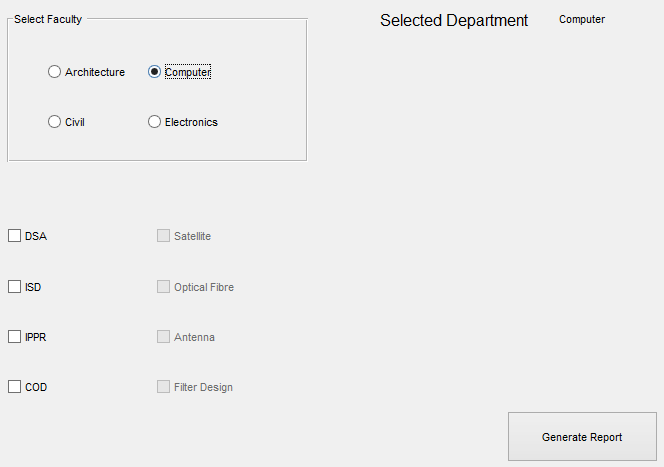
\includegraphics[scale = 0.6]{output_labfour_1.png}\\

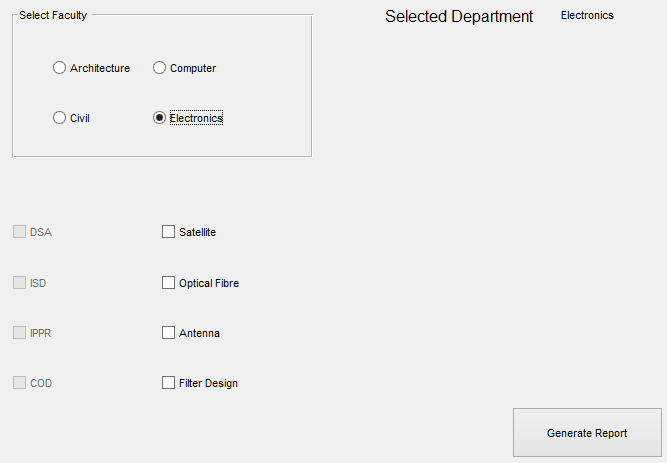
\includegraphics[scale = 0.6]{output_labfour_2.png}
\pagebreak
\section{Conclusion}
Hence, \\
We are familiarized with how GUI operations are performed in Matllab using various functions.
\newpage
%\bibliographystyle{plain}
%\bibliography{biblist}

\end{document}